\chapter{Data analysis framework}
\label{chap:analysisframework}

\section{MIDAS DAQ output in a nutshell}
The main DAQ framework for the Muon g-2 experiment is based on \ac{midas}~\cite{Midas}. The Midas DAQ system is developed at \ac{psi} and \ac{truimf}.
MIDAS event structure is as depicted in Fig.~\ref{fig:MIDASEventStructure}.

\begin{figure}[htbp]
\centering
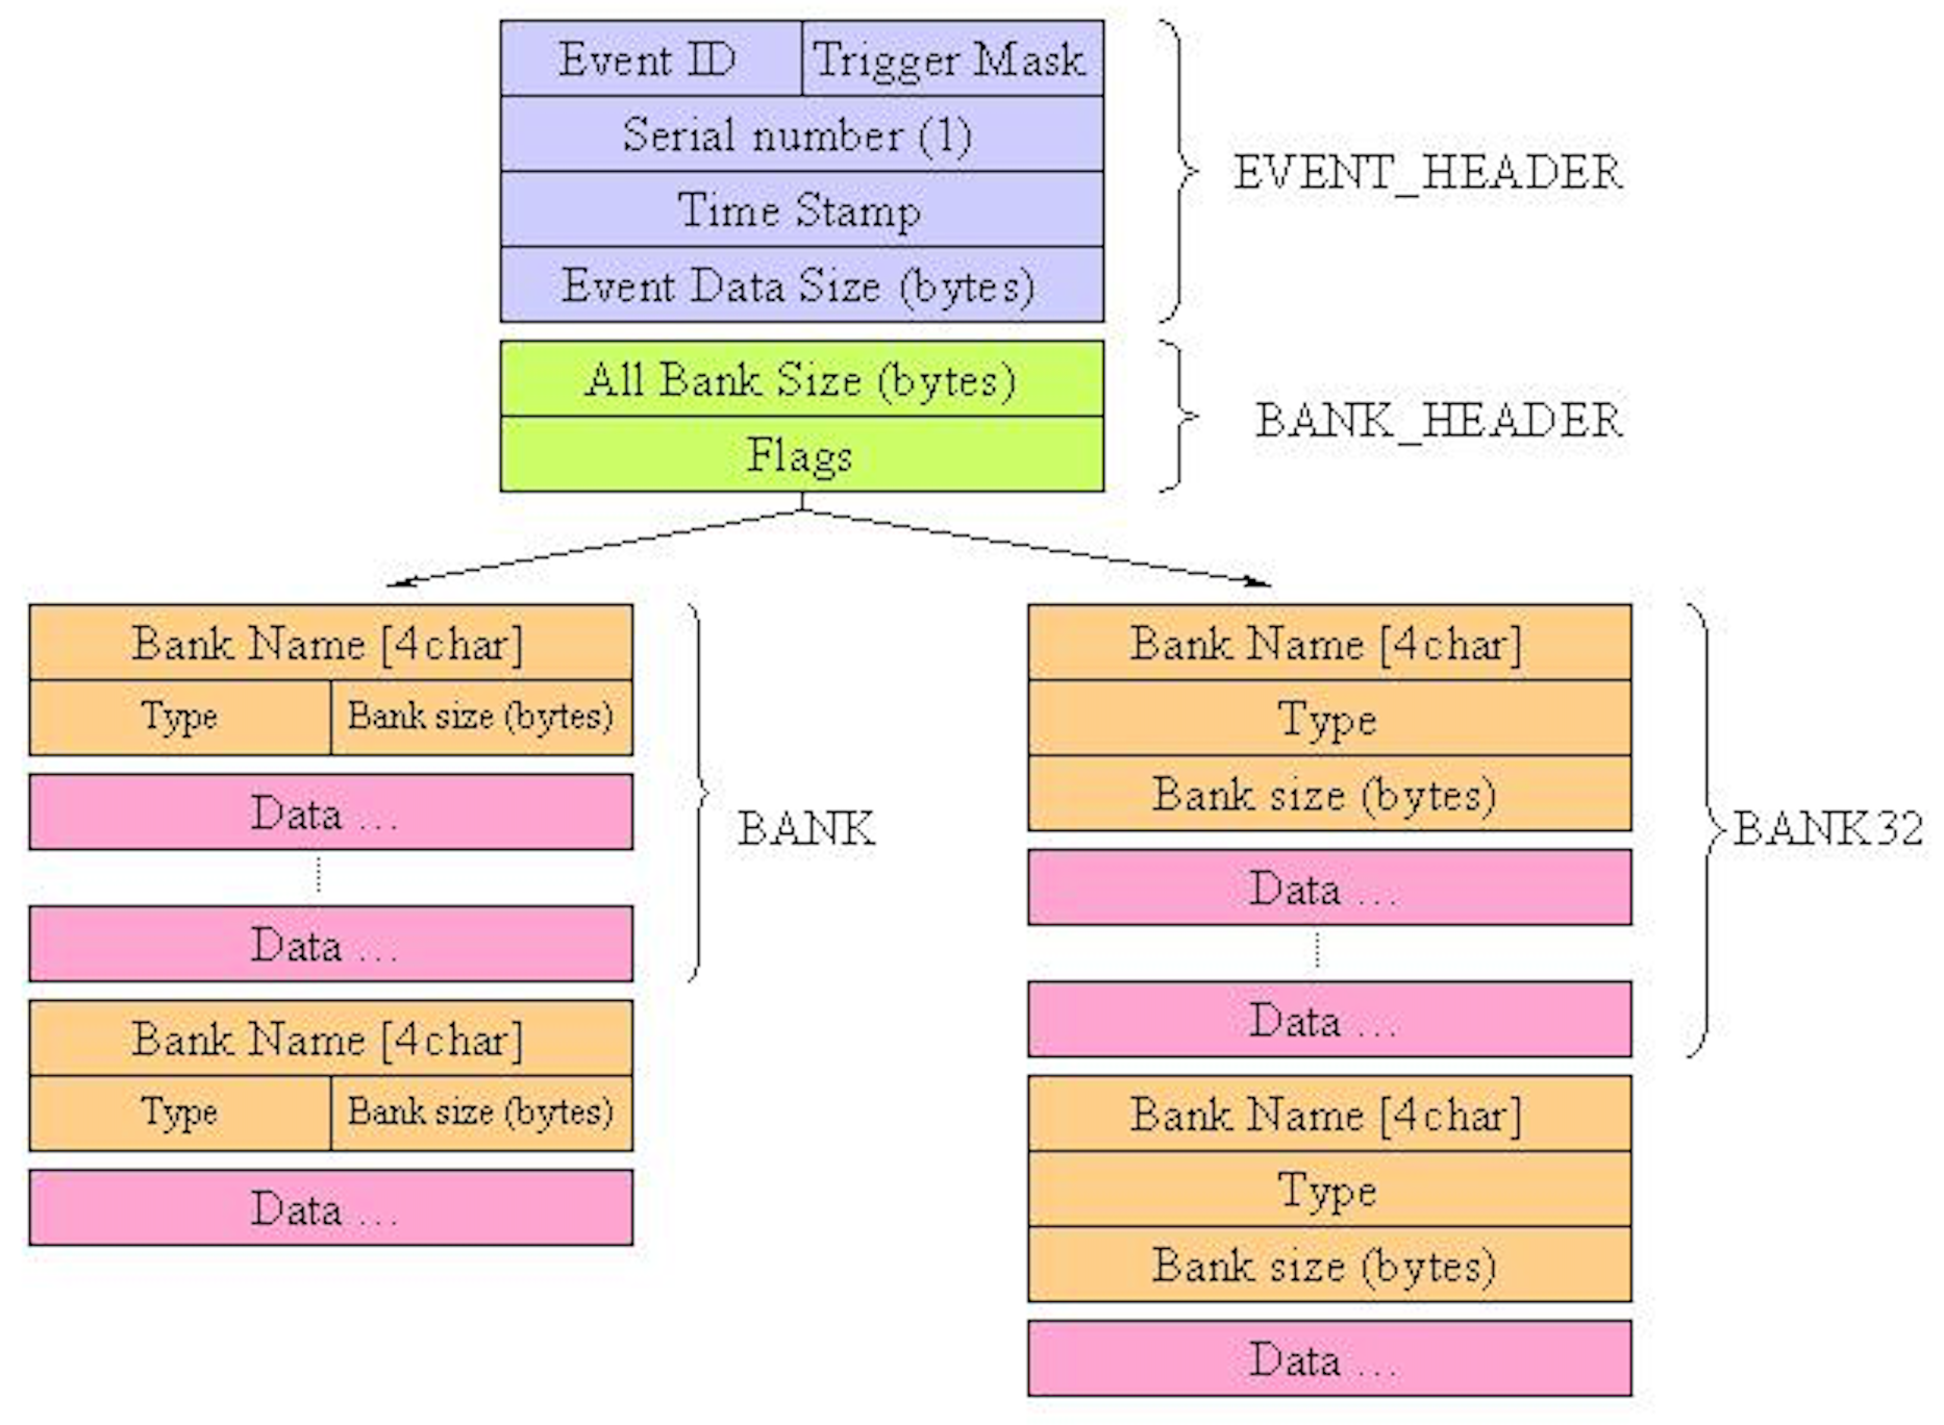
\includegraphics[width=0.6\textwidth]{pics/MIDASEventStructure.pdf} 
\caption{MIDAS event structure. Each event has its header that is followed by the bank header. Then all the banks will appear according the defined order.}\label{fig:MIDASEventStructure}
\end{figure}

\section{Offline framework for the SLAC test beam}

\begin{figure}[htbp]
\centering
%\fbox{\includegraphics[trim=0cm 5.5cm 0cm 5.5cm ,width=0.9\textwidth]{pics/EMShower}} guide line for trimming
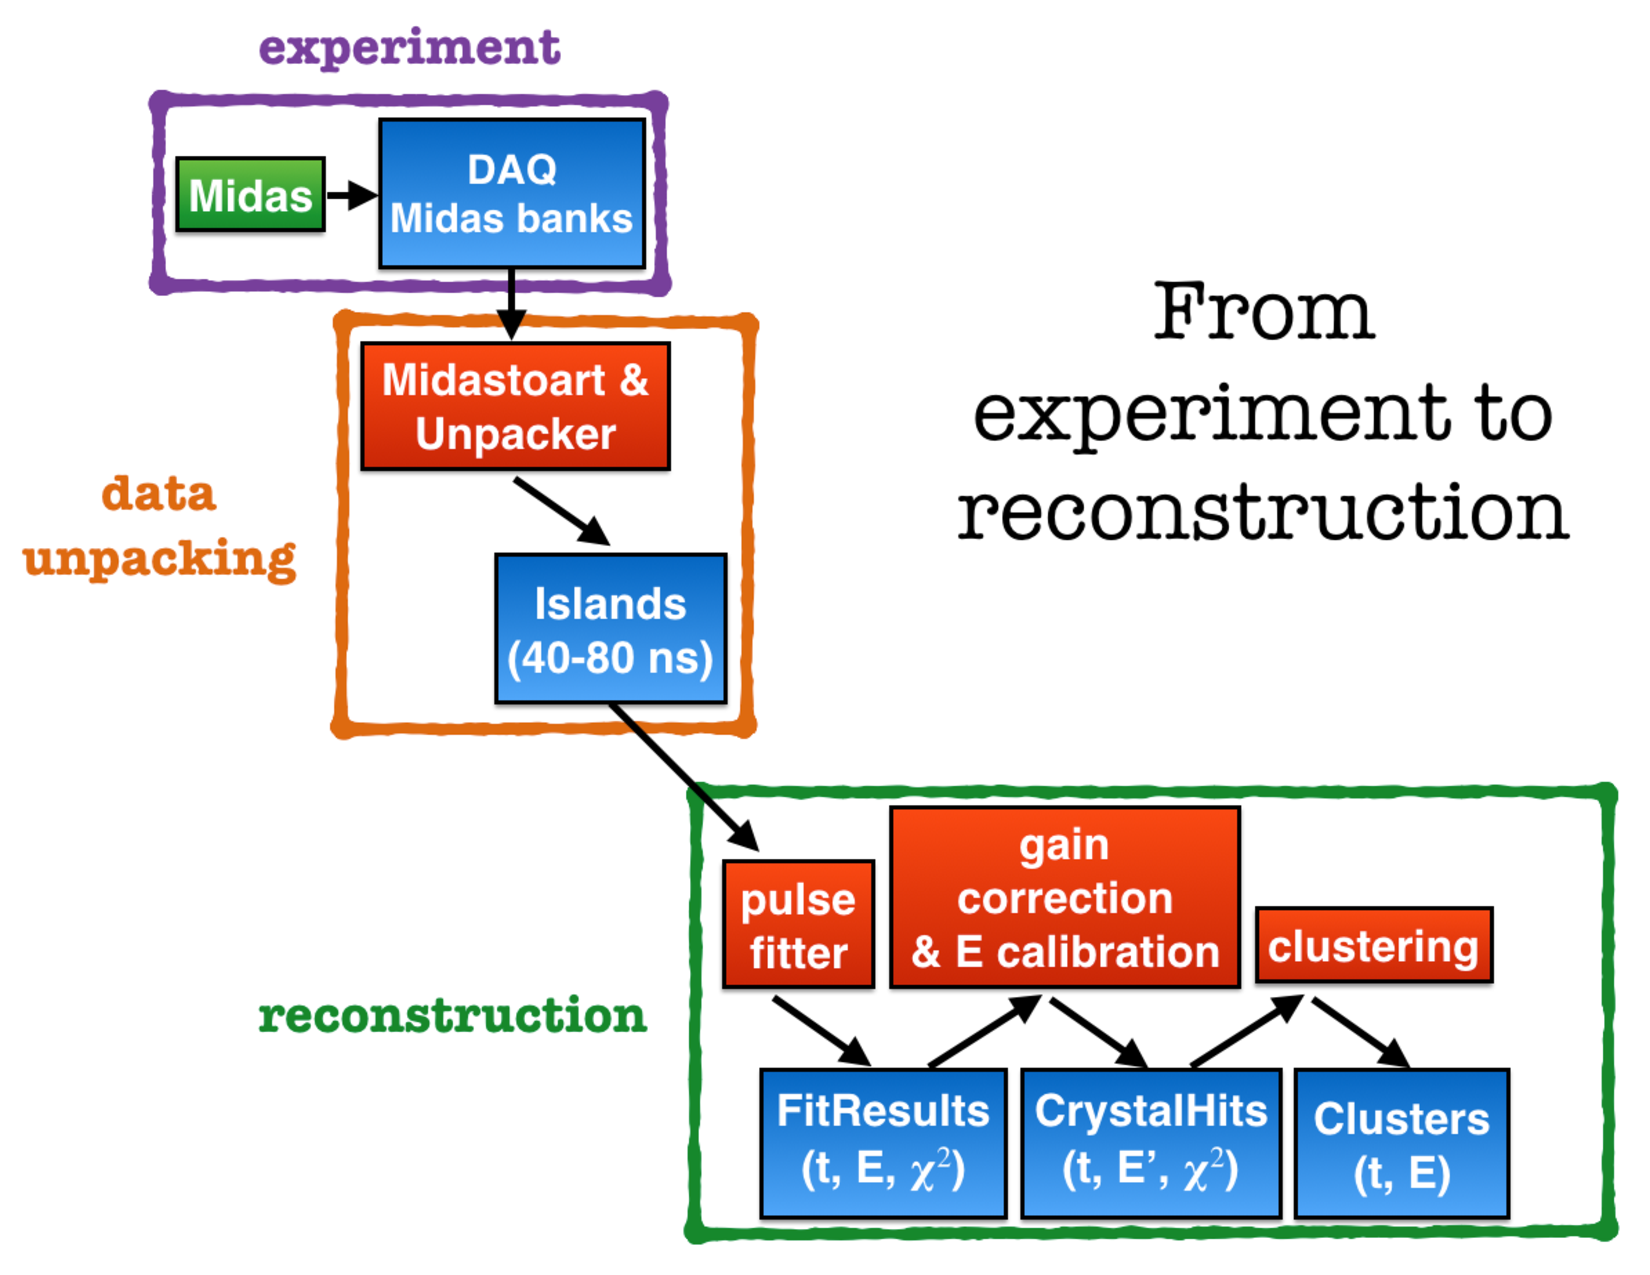
\includegraphics[width=0.7\textwidth]{pics/offline_exp_framework}
\caption{An overview of the Muon g-2 offline framework.}
\label{pic:exp_framework}
\end{figure}

As shown in \fref{pic:exp_framework}, data analysis for this test beam has several components. First we need to convert the raw data stored in a MIDAS file (\verb+.mid+ or \verb+.mid.gz+) to \textit{art} data products stored in an \textit{art} file.
This is handled using \textit{art} framework's modules and is doing nothing more than storing \verb+16-bit+ or \verb+32-bit+ word into \verb+vectors+. Next we unpack these \verb+vectors+
and give them contexts based on the header information stored within the \verb+vectors+. At this step, all the information are stored as data products you are probably familiar with: \verb+RiderArtRecord+,
\verb+IslandArtRecord+, etc. Then reconstruction algorithms are ran through these data products and at the end of the chain each physics objects are reconstructed as clusters.
%
\begin{figure}[htbp]
\centering
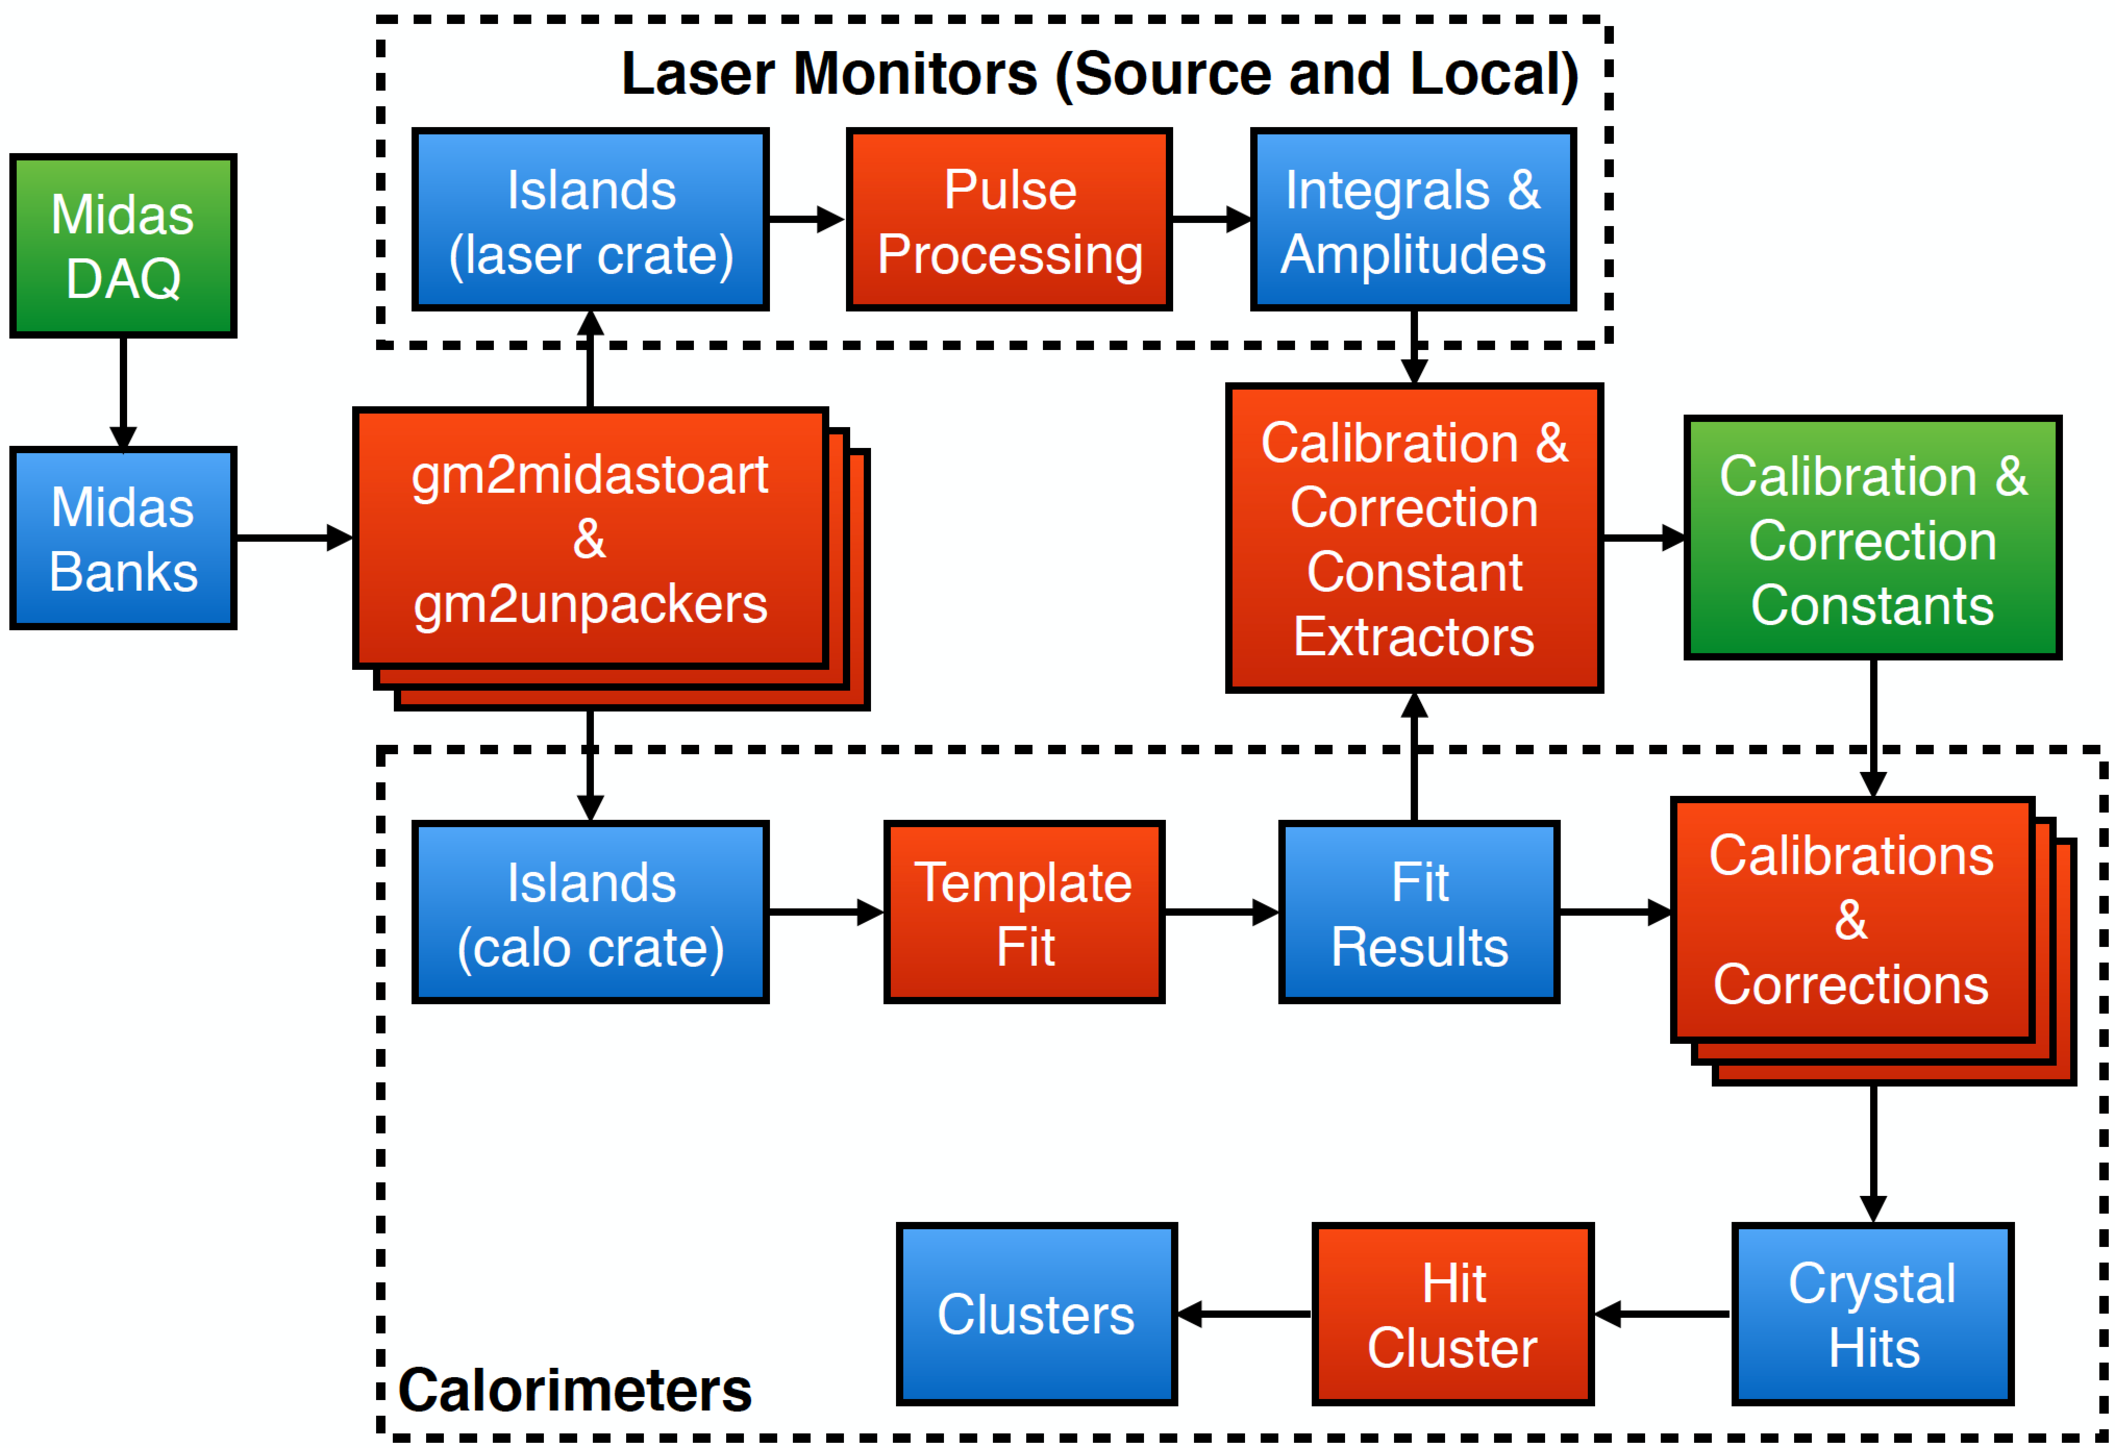
\includegraphics[width=0.7\textwidth]{pics/offline_slac_art_framework}
\caption{Offline \textit{art} framework for the SLAC experimental data.}
\label{pic:art_framework}
\end{figure}
%
The final \textit{art} framework used at SLAC is shown in \fref{pic:art_framework}.

\subsection{Data Acquisition}
Explain the DAQ flow here roughly (from machine trigger to FC7, from FC7 fanout to AMC13 of all the \ac{utca} crates, then from the AMC13 to AMCs(WFD5s) in a crate).

\subsection{Data Unpacking}
The task of unpacking the raw midas data is divided into several \textit{art} modules. First, the Midas banks are converted into TBranches as vectors in the source input module under the repository gm2midastoart.
Then the header information stored in the \verb+CB+ banks is unpacked by the module \verb+HeaderUnpacker+, 
the raw waveforms stored in the \verb+CR+ banks in the calorimeter (fc7, laser) crate is unpacked by the RawUnpacker (LaserRawUnpacker, FC7Unpacker), the chopped islands stored in the \verb+CT+ banks
is unpacked by the IslandUnpacker (LaserUnpacker) and so on. Fhicl file configuration will be explained in the next section.

Unpacking the slow control data like the temperature readout from SCS3000 requires some modification to the gm2midastoart's \verb+MidasBankInput+ module.
The \verb+event id+ for the fast control events is assigned as 1 by the MIDAS DAQ whereas for the slow control it is 11 (\verb+0x000b+ in hex representation).
The bank name for the SLAC2016 setup is \verb+INPT+ and the bank data type is \verb+float+.

\subsection{Reconstruction}
The data reconstruction chain is consisted of 5 modules in series: pulse fitter, energy calibrator, gain corrector, time corrector and hit cluster. Fhicl file configuration will be explained in the next section.